\documentclass[12pt, a4paper]{article}
\usepackage{url,graphicx,tabularx,array,geometry}
\usepackage[utf8]{inputenc}
\usepackage{paralist}
\usepackage{latexsym}
\usepackage{fancyhdr}
\usepackage{ textcomp }
\usepackage{ mathrsfs }
\usepackage{ dsfont }

\pagestyle{fancy}

\usepackage{amsmath}
\usepackage{amsfonts}
\usepackage{amssymb}


\setlength{\parskip}{1ex} %--skip lines between paragraphs
\setlength{\parindent}{0pt} %--don't indent paragraphs

%-- Commands for header
\newcommand{\bs}{\ensuremath{\backslash}}
\renewcommand{\title}[1]{\textbf{#1}\\}
\renewcommand{\line}{\begin{tabularx}{\textwidth}{X>{\raggedleft}X}\hline\\\end{tabularx}\\[-0.5cm]}
\newcommand{\leftright}[2]{\begin{tabularx}{\textwidth}{X>{\raggedleft}X}#1%
& #2\\\end{tabularx}\\[-0.5cm]}
%\linespread{2} %-- Uncomment for Double Space
\begin{document}
\renewcommand{\headrulewidth}{0pt}
\fancyhf{}
\fancyhead[L]{
\leftright{\textbf{Kommunikationssysteme - Serie 1}}{Hannes Strubel, Daniel Schmidt}
\line
}
\fancyfoot[C]{\thepage}

\section*{Kap. Syntax, oben, Aufgabe 2}
\subsection*{Aufgabenstellung}
Streichen Sie in der folgenden Formel so viele Klammern wie möglich, ohne dass sich die Formel ändert:
\begin{equation}
(X_3 \leftrightarrow (\bot \vee (X0 \wedge X_2) \rightarrow ((X0 \wedge X_2) \vee (X_1 \uparrow \neg X_3))))
\end{equation}

Erläutern Sie Ihr Ergebnis.

\subsection*{Lösung}
\begin{equation}
\begin{split}
&(X_3 \leftrightarrow (\bot \vee (X_0 \wedge X_2) \rightarrow ((X_0 \wedge X_2) \vee (X_1 \uparrow \neg X_3))))\\
=^1 &X_3 \leftrightarrow (\bot \vee (X_0 \wedge X_2) \rightarrow ((X_0 \wedge X_2) \vee (X_1 \uparrow \neg X_3)))\\
=^2 &X_3 \leftrightarrow \bot \vee X_0 \wedge X_2 \rightarrow ((X_0 \wedge X_2) \vee (X_1 \uparrow \neg X_3))\\
=^3 &X_3 \leftrightarrow \bot \vee X_0 \wedge X_2 \rightarrow (X_0 \wedge X_2 \vee X_1 \uparrow \neg X_3)\\
=^4 &X_3 \leftrightarrow \bot \vee X_0 \wedge X_2 \rightarrow X_0 \wedge X_2 \vee X_1 \uparrow \neg X_3
\end{split}
\end{equation}

Diese Klammern können weggelassen werden, da
\begin{enumerate}
\item um den gesamten Ausdruck keine Klammer nötig ist.
\item die Junktoren $\leftrightarrow$ und $\rightarrow$ schwächer binden als $\wedge$.
\item $\wedge$ (beziehungsweise $\uparrow$, also $\wedge \neq$) stärker bindet als $\vee$.
\item $\wedge$ stärker bindet als $\rightarrow$.
\end{enumerate}

\section*{Kap. Syntax, unten, 1}
\subsection*{Aufgabenstellung}
Definieren Sie die Funktion size: $F_{AL} \rightarrow \mathds{N}$, die jeder aussagenlogischen Formel ihre Größe, die durch die Anzahl der Knoten des entsprechenden Baumes gegeben ist, zuordnet.

\subsection*{Lösung}
\subsubsection*{Basiszuordnung}
size($\{ \top \}$) = 1\\
size($\{ \bot \}$) = 1\\
size($\{ X_i \}$) = 1 für alle $i \in \mathds{N}$
\subsubsection*{Induktionsregel}
Ist j ein n-stelliger Junktor und $\varphi_0,....,\varphi_{n-1}$ Formeln, so gilt:\\
\begin{equation}
\begin{split}
size(J(\varphi_0,....,\varphi_{n-1})) &= 1 + size(\varphi_0) + ... + size(\varphi_{n-1})\\
&= 1 + \sum^{n-1}_{i=0} size(\varphi_i)
\end{split}
\end{equation}

\section*{Kap. Syntax, unten, 2}
\subsection*{Aufgabenstellung}
Definieren Sie die Funktion conns: $F_{AL} \rightarrow \mathcal{P}(\{ \neg ,\wedge ,\vee ,\rightarrow,\leftrightarrow ,\nleftrightarrow ,\uparrow \})$, die jeder aussagenlogischen Formel die Menge der in ihr vorkommenden Junktoren zuordnet.
\subsection*{Lösung}
\subsubsection*{Basiszuordnung}
conns($\{ \top \}$) = \{\}\\
conns($\{ \bot \}$) = \{\}\\
conns($\{ X_i \}$) = \{\} für alle $i \in \mathds{N}$
\subsubsection*{Induktionsregel}
Ist j ein n-stelliger Junktor und $\varphi_0,....,\varphi_{n-1}$ Formeln, so gilt:\\
\begin{equation}
\begin{split}
conns(J(\varphi_0,....,\varphi_{n-1})) &= J \cap conns(\varphi_0) \cap ... \cap conns(\varphi_{n-1})\\
&= J \cap \bigcap_{i \in \mathds{N}}(conns(\varphi_i))
\end{split}
\end{equation}

\section*{Kap. Syntax, unten, 5}
\subsection*{Aufgabenstellung}
Sehen Sie eine Möglichkeit, in die Aussagenlogik auch Junktoren mit unendlicher Stelligkeit aufzunehmen? – Wenn ja, wie könnte das aussehen? Wenn nein, warum nicht?
\subsection*{Lösung}
Ja. Wenn man einen Junktor J hätte und diesen so definiert, dass f.a. $X_i, i \in \mathds{N}$ gilt:
\begin{equation}
X_0 J X_1 J X_2 = ((X_0 J X_1) J X_2)
\end{equation}
In diesem Fall eine unendlichstellige Variante dieses Junktors in eine 2 stellige Variante überführen, die dann einen unendlichen Teilbaum hat. Da diese nicht ausgeschlossen sind sollte es keine Probleme geben.

\section*{Kap. Semantik, 1}
\subsection*{Aufgabenstellung}
Werten Sie die Formel $X_0 \wedge X_1 \leftrightarrow (\neg X_0 \vee X_1)$ schrittweise unter einer Belegung $\beta$, für die $\beta(X_0)=0$ und $\beta(X_1)=1$ gilt, aus. Zeichnen Sie das zugehörige Diagramm.
\subsection*{Lösung}
\begin{equation}
\begin{split}
&X_0 \wedge X_1 \leftrightarrow ( \neg X_0 \vee X_1)\\
&0 \wedge 1 \leftrightarrow (\neg 0 \vee 1)\\
&0 \leftrightarrow (\neg 0 \vee 1)\\
&0 \leftrightarrow (1 \vee 1)\\
&0 \leftrightarrow 1\\
&0
\end{split}
\end{equation}
Das dazugehörige Baumdiagramm sieht so aus:
\begin{figure}[H] 
		\centering
		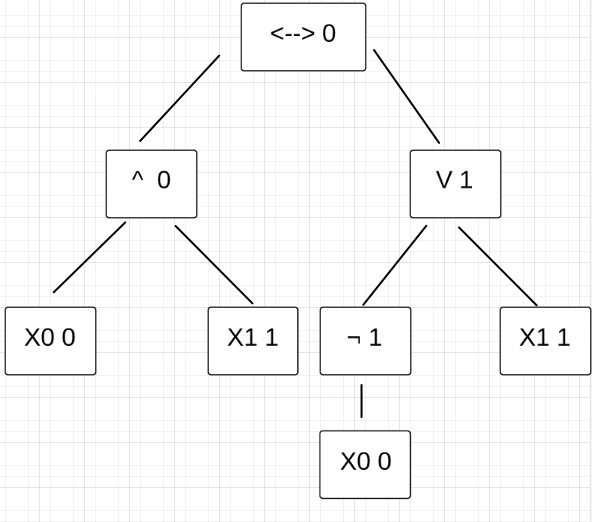
\includegraphics[page=1, width=0.9\textwidth]{a1-sem}
		\caption{Baumdiagramm} 
		\label{Baumdiagramm}
\end{figure}

\end{document}